\section{Methodology}\label{methodology}

To construct the initial seq2seq model, the PyTorch neural network library for python was used. Recall from Section~\ref{tf} that other state-of-the-art solutions are not able to implement dynamic teacher forcing methods due to the fact that the computational graph must be pre-defined before inference. 

Specifically, I used an open source seq2seq pytorch jupyter notebook for neural machine translation\footnote{Available at: https://github.com/jph00/part2/blob/master/translate-pytorch.ipynb} as the base model. Several modifications were made to this model, including the implementation of bidirectional RNNs and various teacher forcing methods, as well as redefining input and output parameters for the specific task of headline-length abstractive summarization.

\subsection{Data and Preprocessing}
The dataset used for this project and all other state-of-the-art models for this task is The University of Pennsylvania Linguistic Data Consortium's Annotated English Gigaword Corpus\footnote{https://catalog.ldc.upenn.edu/ldc2012t21}, graciously provided via scholarship, which contains over four million article-headline pairs from seven news publications between 1994 to 2010. Specifically, the LDC data was structured as 1,011 gzipped XML files, each file representing a month of articles from one of the news sources. Because the data was delivered via an external hard drive and I did not have access to a University computer, the dataset had to be processed on a 2015 Macbook Pro. Unfortunately, this meant that the 154 largest XML files had to be discarded due to the computers inability to store their parsed XML trees in memory. It was decided that the dataset should be pared back to \~100,000 pairs, so 120 articles were sampled randomly from each of the remaining 857 files.

To address the file format, the LXML library was used to unzip and parse the XML tree. After randomly shuffling all of the child nodes of the XML tree, a series of regex substitutions were used to strip the unnecessary part-of-speech tags which accompanied every word in the dataset to transform the necessary data into raw text. It must be noted that all state-of-the-art headline generation models currently only use the first sentence of the article as input, as this is generally found to be sufficient to generate headlines~\cite{Liu2016}. I maintained this convention within this project, so any reference to an article is only to the first sentence of said article in practice.

One drawback of the LDC dataset is that there is a non-negligable amount of nonsensical headlines that also happen to be very long. To combat this, I restricted the length of headlines to 30 words and articles to a length of 50 words, the same criteria used in the highest-performing model~\cite{Liu2016}. Any pairs that did not meet both of these criteria were discarded, resulting in a 20.7\% discard rate. The remaining 79.3\% randomly sampled, fully preprocessed article/headline pairs were then placed into respective lists. The code for extracting the data can be found in Appendix~\ref{app:extraction}.

The sentences were then turned into word indexes within a vocabulary list for every headline/article pair, keeping the 200,000 most common words and substituting all other words with an $<UNK>$ token, for unknown. This practice is in line with the highest-performing state-of-the-art model~\cite{Liu2016}. A $<SOS>$, start of sentence pad, or index 1, was added to the start of every pair. Then each sentence was padded with the $<PAD>$ token, or index 0, on the ends to make each input and output the same length. The data was then split 90\% training, 10\% test. Lastly, each word was also linked with its associated 100-dimensional GLoVe embedding (See Sec.~\ref{emb}) if an embedding existed for the word. Otherwise, a random initialization was created for the word to be trained by the model. Unfortunately, due to licensing constraints, I cannot share the contents of any of the data, but the processed, indexed pairs can be seen in Figure~\ref{fig:procd}.

\begin{figure}[h]
  \centering
  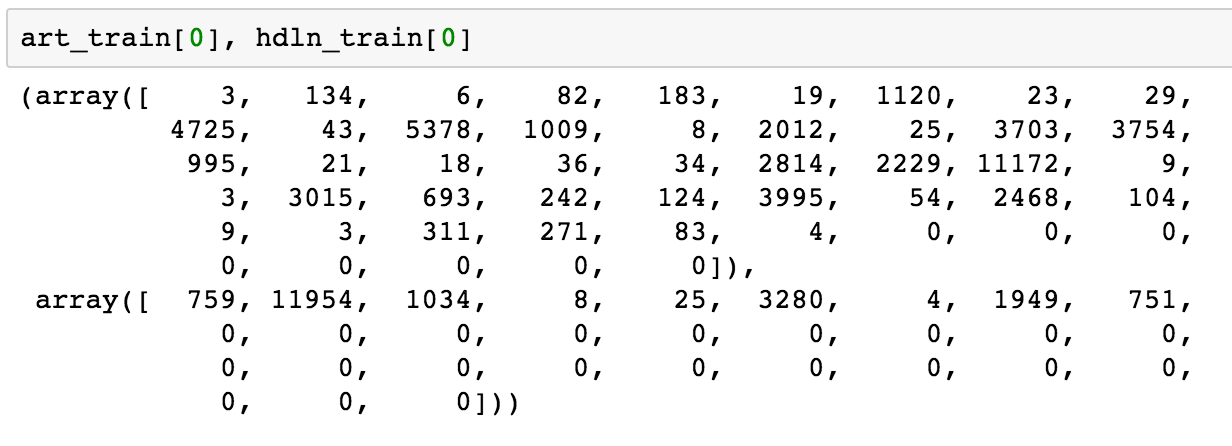
\includegraphics[width=.85\textwidth]{procd}
  \caption{A preprocessed headline and article pair with zero-padding.}
  \label{fig:procd}
\end{figure}

\subsection{Difficulties and RNN Architecture Adjustments}
When initially setting out to research this issue of teacher forcing, several large issues presented themselves. First and foremost, training DNNs can take significant resources, some using more than 300 GPUs simultaneously~\cite{Silver2016}. For my specific task,attempts at adhereing to state-of-the-art model parameters revelaed that fully training such a model from scratch would take over 10 days per experiment on a single GPU, confirmed by~\cite{Nallapati2016a}. Furthermore, because teacher forcing is a method used during model training, pretrained models could not be used. Therefore, modifications were required to achieve results within a reasonable time.

The current state-of-the-art headline generation model uses four bidirectional encoder layers, four bidirectional decoder layers, a word embedding size of 128, and 256 hidden nodes per LSTM~\cite{Liu2016}. The greater one can increase any of these dimensions, the greater the model's learned complexities between inputs, outputs and intra-word relationships at the cost of computational requirement for both training and evaluating. This model was trained on multiple GPUs (though the exact number is not specified) and appeared that it would take weeks to converge on a single GPU through a short test run. Because of this, the same general seq2seq architecture was maintained, but all dimensionalities reduced to the following: one layer encoder, one layer decoder, word embedding size of 300, and hidden size of 128 nodes per LSTM. With these parameters, models appear to converge within approximately four hours on the University's Titan X (Pascal) GPU instance (Thadeus machine). Due to this decrease in model complexity, one cannot hope for comparative results to state-of-the-art, so instead, results for various teacher forcing methods will only be judged relative to one another.

As a final precaution, it must be noted that these models are learning sequence generation from headlines that have been chosen by the publications, meaning they are still subject to bias. The idea, however, is that by generalizing well enough amongst a large dataset, biases will naturally be mitigated. I think this is likely incorrect, and that Recurrent Neural Networks will pick up trace biases by the very nature of their capability to understand and interpret nuance to such an incredible degree of dimensionality. That said, developing effective abstractive techniques is the first step in a long road towards the mitigation of editorial bias in online news, and seq2seq is currently at the forefront of development in this arena.

\subsection{Experiment Set-up}
Recall from Section~\ref{grad} that a learning rate is picked by the DNN engineer to change all the weights within the network. This learning rate needs to be decreased as the model gets closer and closer to convergence in a process called learning rate annealing. It was found that 40,000 cycles of generating a random batch of 128 examples, annealed every 5,000 - 10,000 cycles, was adequate for model convergence. The first two sets of 5,000 batches had a learning rate of 0.003; the second two sets of 5,000 had learning rates of 0.001; the third two sets of 5,000 batches had learning rates of 0.0003; the next set of 5,000 had a learning rate of 0.0001; the last set of 5,000 had a learning rate of 0.00003. This progression can be seen clearly in the \texttt{multi\_train} function in Appendix~\ref{app:train}.

I trained seven different models on these teacher forcing (TF) methods: graduated, graduated-reset, 100\%, 75\%, 50\%, 25\%, and 0\%. For the graduated model, the chance of teacher forcing started at 100\% and decreased linearly over the course of the entire 40,000 batches of training until eventually 0\% teacher forcing was allowed by the last batch. Graduated-reset would gradually decrease the amount of teacher forcing over every 5,000 batches, so full teacher forcing was reset to 100\% and tapered to 0\% for each of the 8 sets of 5,000 batches. The differences can be further investigated by referencing the \texttt{trainEpochs} and \texttt{fullgraduated\_trainEpochs} functions in Appendix~\ref{app:train}. The various percentages listed above provided the associated teacher forcing probability throughout the entire training period.

To ensure that the training and test splits were not disproportionately influencing one TF method over another by chance, I trained and tested every model 3 different times on randomized data splits. In doing so, I was able to ascertain that all TF methods on all three tests were statistically similar, and consequently any of the test results could be used for further analysis. See Section~ref{stat} for details.

\subsection{Evaluation Metrics}
When evaluating the effectiveness of various teacher forcing methods, there are two main metrics to condiser: loss over time and ROUGE.

\subsubsection{ROUGE}\label{method:rouge}
Firstly, to judge generative performance, the metric used in all previous explorations of headline-length text summarization~\cite{Rush2015,Chopra2016,Nallapati2016a,Liu2016,See2017}: Recall-Oriented Understudy for Gisting Evaluation, or ROUGE~\cite{Lin2004}, will likewise be used for this project. There are two ROUGE metrics of interest: ROUGE-1, ROUGE-2. For the purposes of this task, ROUGE-1 measures the overlap of each word between the generated summary and the label. ROUGE-2 measures the overlap of adjacent words between the generated summary and the correct label. The top ROUGE scores for each state-of-the-art abstractive model can be compared in Table~\ref{tab:rouge}.
\begin{table}[h]
  \begin{center}
    \begin{tabular}{ | l l | c | c | }
      \hline
      & & ROUGE-1 & ROUGE-2 \\
      \hline
      Rush & [Facebook] & 29.78 & 11.89 \\
      Chopra & [Facebook] & 33.78 & 15.97 \\
      Nallapati & [IBM] & 35.30 & 16.64 \\
      Liu & [Google Brain] & 42.56 & 23.12 \\
      \hline
    \end{tabular}
    \caption{ROUGE-1 and ROUGE-2 scores for top performing abstractive models}
    \label{tab:rouge}
  \end{center}
\end{table}
By measuring these values, we can ascertain how close the generated output was to matching words and word pairs from the beginning. While this metric is quite unsophisticated and does not well convey actual comprehension, it is the metric used by all other headline-length abstractive summarization researchers to judge performance and consequently is the metric chosen to be used here.

\subsubsection{Loss Over Time}
Evaluating visualizations of loss over the training period is another important metric in judging the effectiveness of various TF methods. Recall from Section~\ref{tf} that the reason teacher forcing became a topic of discussion in the first place was the idea that, at the beginning of model training, the model would be generating the wrong output nearly every time. If this incorrect output was constantly fed into the decoder state to predict the next time step, all training afterwards is unhelpful. This would result in far longer convergence times. So, the amount of time it takes for a model to converge is a critical part of the motivation behind teacher forcing. Consequently, the average loss over time was recorded and used to compare the various teacher forcing techniques.

\subsection{Statistical Analysis and Data Visualization}\label{stat}
To compare and contrast the results of the various TF methods from the three different tests, I used the Kruskal-Wallis Test~\cite{Kruskal1952}, which tests whether a number of samples are statistically probable to originate from the same distribution. These results can be found in Section~\ref{results}. As all TF methods over all three tests returned probable to have come from the same distribution, it is safe to assume that all TF methods from all three tests are representative of a general trend, and consequently further analysis only needed to be carried out on one of the tests. To visualize the skewed ROUGE distributions, I created histograms and Q-Q plots using R.

For computing average ROUGE values, I could not discern the methodology used by any of the state-of-the-art researchers. As such, I used what I felt was appropriate given the data distribution. That said, for skewed datasets, the median is typically used and was initially attempted for this analysis. However, the Wilcoxon pseudo-median values gave wildly inaccurate results for ROUGE-2. It would appear that non-normal median-distributed data was not properly accounting for ROUGE values of zero, a statistic that is very important to this specific problem. Consequently, bootstrapping~\cite{Davidson2003}, a mean-centric resampling technique, was used to compute these averages instead.

To test for statistically significant differences between the data, the Wilcoxon test~\cite{Wilcoxon1945} was used. This is a method used for paired difference testing on non-normal data distributions. The values reported are probabilities (p-values) that the differences in median of the compared TF methods is 0. This means that smaller p-values make it less of a possibility that the compared means are in fact the same and no statistical significance exists between them. A p-value $\leq$ 0.05 (5.0E-02) makes the differences statistically significant. Wilcoxon probabilities were calculated relative to three different benchmarks:  all TF methods relative to no TF, all TF methods relative to 100\% TF, and graduated compared to reset-graduated as a matter of academic interest.

Lastly, a look at loss over time is done as a second evaluation metric, again with only one of the test results. The loss and time information was collected in lists during training. These were then plotted using matplotlib, a MATLAB-esque plotting program for python and heavily used in jupyter notebooks. These plots have been provided in Section~\ref{loss}.